\documentclass[../main.tex]{subfiles}

\begin{document}

% exercise 1.1

\section{}

\begin{multicols}{2}
  \begin{itemize}
    \item 10
    \item 12
    \item 8
    \item 3
    \item 6
    \item a (with value 3)
    \item b (with value 4)
    \item 19
    \item \#f (true)
    \item 4
    \item 16
    \item 6
    \item 16
  \end{itemize}
\end{multicols}

% exercise 1.2

\section{}

\begin{lstlisting}
(/ (+ 5
      4
      (- 2
         (- 3
            (+ 6
               (/ 4 3)))))
   (* 3
      (- 6 2)
      (- 2 7)))
\end{lstlisting}

% exercise 1.3

\section{}

\begin{lstlisting}
(define (min2 a b)
  (if (< a b)
      a
      b))
(define (min3 a b c)
  (min2 a
        (min2 b c)))
(define (square x)
  (* x x))
(define (f a b c)
  (- (+ (square a)
        (square b)
        (square c))
     (square (min3 a b c))))
\end{lstlisting}

% exercise 1.4

\section{}

If b is positive, evaluate \lstinline{(- a b)} (i.e. a - b), otherwise evaluate \lstinline{(+ a b)} (i.e. a + b).

% exercise 1.5

\section{}

\subsection*{Applicative-order Evaluation}

\begin{lstlisting}
(test 0 (p)) ->
(test 0 (p)) ->
(test 0 (p)) ->
(test 0 (p)) ->
......
\end{lstlisting}

In applicative-order evaluation, a procedure is not reduced until all its arguments are evaluated. Thus the expression \lstinline{(p)} is constantly being expanded into itself over and over again while the procedure \lstinline{test} can never get the chance to be reduced.

\subsection*{Normal-order Evaluation}

\begin{lstlisting}
(test 0 (p)) ->
(if (= 0 0) 0 (p)) ->
0
\end{lstlisting}

In normal-order evaluation, a procedure's arguments are not evaluated until they're needed, which means the procedure is always reduced until it only involves primitive operators before its arguments are evaluated. Due to the special evaluation rule of \lstinline{if} where the alternative expression is not evaluated if the predicate expression is evaluated to be true, the function \lstinline{test} returns 0 before \lstinline{(p)} gets the chance to be evaluated.

% exercise 1.6

\section{}

The program will run infinitely until it runs out of memory.

\lstinline{if} has a special evaluation rule where either the consequent or the alternative expression is evaluated depending on the value of the predicate expression. In the implementation of Newton's Method, the procedure should immediately return current value when the value is good enough, and here's where \lstinline{if} comes in: if the requirement is met, the recursive call is not made.
 
But the program using \lstinline{new-if} always evaluates both the consequent and the alternative expression, causing the procedure to recursively call itself infinitely.

% exercise 1.7

\section{}

For very small numbers, the threshold value 0.001 is too large to tell if current estimation is close enough to real value.

\lstinline{(sqrt 0.00000001)} returns 0.03125, while 0.0001 is the real value.

For very large numbers, the precision is lost during calculation, hence the estimation can never get close enough ('close' defined by the threshold value 0.001) to real value.

\lstinline{(sqrt (expt 10 150))} fails to return within a reasonable amount of time.

Code after improvement:

\begin{lstlisting}
(define (sqrt-iter guess last x)
  (if (enough? guess last)
      guess
      (sqrt-iter (improve guess x)
                 guess
                 x)))
(define (improve guess x)
  (average guess
           (/ x guess)))
(define (average x y)
  (/ (+ x y)
     2))
(define (enough? guess last)
  (< (/ (abs (- guess last))
        last)
     0.001))
(define (sqrt x)
  (sqrt-iter 1.0 x x))
\end{lstlisting}

After improvement, function calls mentioned above return 1e-4 and 1e75 respectively.

% exercise 1.8

\section{}

\begin{lstlisting}
(define (cbrt-iter guess last x)
  (if (enough? guess last)
      guess
      (cbrt-iter (improve guess x)
                guess
                x)))
(define (improve guess x)
  (/ (+ (/ x
           (* guess guess))
        (* guess 2))
     3))
(define (enough? guess last)
  (< (/ (abs (- guess last))
        last)
     0.001))
(define (cbrt x)
  (cbrt-iter 1.0 x x))
\end{lstlisting}

% exercise 1.9

\section{}

\begin{lstlisting}
(+ 4 5)
(inc (+ 3 5))
(inc (inc (+ 2 5)))
(inc (inc (inc (+ 1 5))))
(inc (inc (inc (inc (+ 0 5)))))
(inc (inc (inc (inc 5))))
(inc (inc (inc 6)))
(inc (inc 7))
(inc 8)
9
\end{lstlisting}

The process is recursive.

\begin{lstlisting}
(+ 4 5)
(+ 3 6)
(+ 2 7)
(+ 1 8)
(+ 0 9)
9
\end{lstlisting}

The process is iterative.

% exercise 1.10

\section{}

\begin{lstlisting}
(A 1 10)
(A 0 (A 1 9))
(A 0 (A 0 (A 1 8)))
...
(A 0 (A 0 (A 0 (A 0 (A 0 (A 0 (A 0 (A 0 (A 0 (A 1 1))))))))))
(A 0 (A 0 (A 0 (A 0 (A 0 (A 0 (A 0 (A 0 (A 0 2)))))))))
(A 0 (A 0 (A 0 (A 0 (A 0 (A 0 (A 0 (A 0 (* 2 2)))))))))
(A 0 (A 0 (A 0 (A 0 (A 0 (A 0 (A 0 (A 0 4))))))))
(A 0 (A 0 (A 0 (A 0 (A 0 (A 0 (A 0 (* 2 4))))))))
(A 0 (A 0 (A 0 (A 0 (A 0 (A 0 (A 0 8)))))))
...
(A 0 512)
(* 2 512)
(1024
\end{lstlisting}

\begin{lstlisting}
(A 2 4)
(A 1 (A 2 3))
(A 1 (A 1 (A 2 2)))
(A 1 (A 1 (A 1 (A 2 1))))
(A 1 (A 1 (A 1 2)))
(A 1 (A 1 (A 0 (A 1 1))))
(A 1 (A 1 (A 0 2)))
(A 1 (A 1 (* 2 2)))
(A 1 (A 1 4))
(A 1 (A 0 (A 1 3)))
(A 1 (A 0 (A 0 (A 1 2))))
(A 1 (A 0 (A 0 (A 0 (A 1 1)))))
(A 1 (A 0 (A 0 (A 0 2))))
(A 1 (A 0 (A 0 (* 2 2))))
(A 1 (A 0 (A 0 4)))
(A 1 (A 0 (* 2 4)))
(A 1 (A 0 8))
(A 1 (* 2 8))
(A 1 16)
...
65536
\end{lstlisting}

\begin{lstlisting}
(A 3 3)
(A 2 (A 3 2))
(A 2 (A 2 (A 3 1)))
(A 2 (A 2 2))
(A 2 (A 1 (A 2 1)))
(A 2 (A 1 2))
(A 2 (A 0 (A 1 1)))
(A 2 (A 0 2))
(A 2 (* 2 2))
(A 2 4)
...
65536
\end{lstlisting}

\begin{itemize}
\item \lstinline{(f n)} equals \lstinline{(A 0 n)} equals \lstinline{(* 2 n)} which computes 2n for positive n.
\item \lstinline{(g n)} equals \lstinline{(A 1 n)} equals \lstinline{(A 0 (A 1 (- n 1)))} equals \lstinline{(* 2 (A 1 (- n 1)))} (which, though, is not the way it's evaluated). In the basic case \lstinline{(A 1 1)} returns 2, thus \lstinline{(g n)} computes $2^n$ for positive n.
\item \lstinline{(h n)} equals \lstinline{(A 2 n)} equals \lstinline{(A 1 (A 2 (- n 1)))} equals \lstinline{(expt 2 (A 2 (- n 1)))} (which, though, is not the way it's evaluated). In the basic case \lstinline{(A 2 1)} returns 2. Informally, \lstinline{(h n)} computes $2^{2^{2^{...}}}$ where the number of 2 is n. The concise definition can be given recursively as follows: \lstinline{(h 1)} returns 2 for 1, and returns \lstinline{(expt 2 (h (- n 1)))} for n larger than 1.
\end{itemize}

% exercise 1.11

\section{}

Recursive version:

\begin{lstlisting}
(define (f n)
  (if (< n 3)
      n
      (+ (f (- n 1))
         (* 2 (f (- n 2)))
         (* 3 (f (- n 3))))))
\end{lstlisting}

Iterative version:

\begin{lstlisting}
(define (f n)
  (define (f-iter n curr a b c)
    (if (= curr n)
        a
        (f-iter n (+ 1 curr) (+ a (* 2 b) (* 3 c)) a b)))
  (if (< n 3)
      n
      (f-iter n 2 2 1 0)))
\end{lstlisting}

% exercise 1.12

\section{}

\begin{lstlisting}
(define (pascal line row)
  (if (or (= row 1)
          (= row line))
      1
      (+ (pascal (- line 1) (- row 1))
         (pascal (- line 1) row))))
\end{lstlisting}

% exercise 1.13

\section{}

Let $\phi = \frac{1 + \sqrt{5}}{2}$, $\psi = \frac{1 - \sqrt{5}}{2}$.

Let $f(n) = \frac{\phi ^ n - \psi ^ n}{\sqrt{5}}$. Then there are $f(0) = 0$, $f(1) = 1$.

For any n larger than 1, consider $f(n - 1)$ and $f(n - 2)$:

\begin{align*}
f(n-1) + f(n-2) &= \frac{\phi^{n-1} + \phi^{n-2}-(\psi^{n-1}+\psi^{n-2})}{\sqrt{5}} \\
                &= \frac{(1+\phi)\phi^{n-2}-(1+\psi)\psi^{n-2}}{\sqrt{5}} \\
                &= \frac{\phi^2\phi^{n-2}-\psi^2\psi^{n-2}}{\sqrt{5}} \\
                &= \frac{\phi^n-\psi^n}{\sqrt{5}} \\
                &= f(n)
\end{align*}

In basic cases $f(0)=Fib(0) and f(1)=Fib(1)$. Given $f(n-2)=Fib(n-2)$ and
 $f(n-1)=Fib(n-1)$ there is
 $f(n)=f(n-1)+f(n-2)=Fib(n-1)+Fib(n-2)=Fib(n)$. Therefore, Fib(n)=f(n)
 stands for all non-negative integer n.

Besides, there is $\left|\frac{\psi^n}{\sqrt{5}}\right|<\frac{1}{2}$:

\begin{align*}
\left({\frac{\psi^n}{\sqrt{5}}}\right)^2 &= \frac{\left({\frac{1-\sqrt{5}}{2}}\right)^{2n}}{5} \\
&= \frac{\left({\frac{3-\sqrt{5}}{2}}\right)^{n}}{5} \\
&\leq \frac{\left(\frac{1}{2}\right)^n}{5} \\
&\leq \frac{1}{5} \\
&< \frac{1}{4}
\end{align*}

Since $Fib(n)=\frac{\phi^n}{\sqrt{5}}+\frac{\psi^n}{\sqrt{5}}$, $Fib(n)$ is the closest
 integer to $\frac{\phi^n}{\sqrt{5}}$.

% exercise 1.14

\section{}

Since the tree is really large, here only the process of \lstinline{(count-change 4)} is illustrated.

\vspace{5mm}
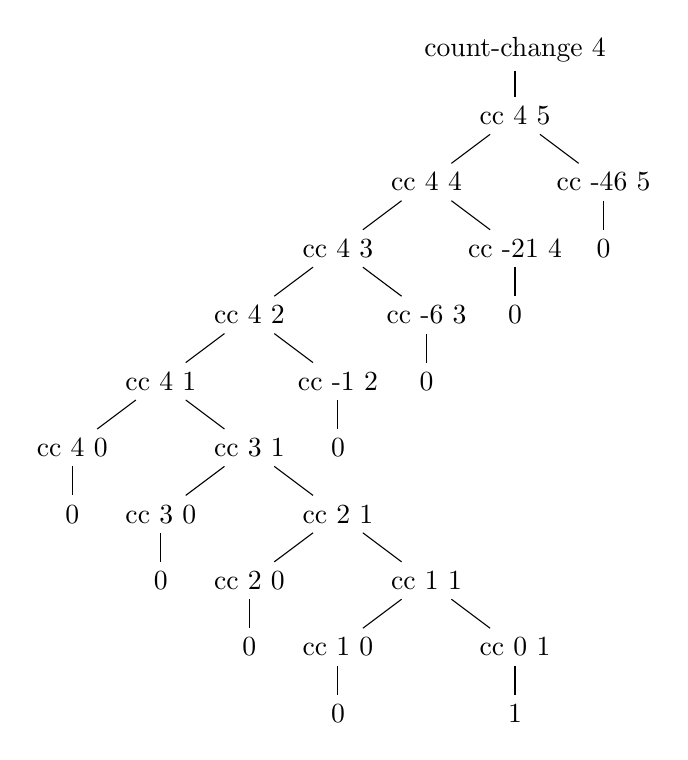
\begin{tikzpicture}[sibling distance=64pt, level distance=24pt]

\node{\lstinline{count-change 4}}
  child{node{\lstinline{cc 4 5}}
    child{node{\lstinline{cc 4 4}}
      child{node{\lstinline{cc 4 3}}
        child{node{\lstinline{cc 4 2}}
          child{node{\lstinline{cc 4 1}}
            child{node{\lstinline{cc 4 0}}
              child{node{\lstinline{0}}}
            }
            child{node{\lstinline{cc 3 1}}
              child{node{\lstinline{cc 3 0}}
                child{node{\lstinline{0}}}
              }
              child{node{\lstinline{cc 2 1}}
                child{node{\lstinline{cc 2 0}}
                  child{node{\lstinline{0}}}
                }
                child{node{\lstinline{cc 1 1}}
                  child{node{\lstinline{cc 1 0}}
                    child{node{\lstinline{0}}}
                  }
                  child{node{\lstinline{cc 0 1}}
                    child{node{\lstinline{1}}}
                  }
                }
              }
            }
          }
          child{node{\lstinline{cc -1 2}}
            child{node{\lstinline{0}}}
          }
        }
        child{node{\lstinline{cc -6 3}}
          child{node{\lstinline{0}}}
        }
      }
      child{node{\lstinline{cc -21 4}}
        child{node{\lstinline{0}}}
      }
    }
    child{node{\lstinline{cc -46 5}}
      child{node{\lstinline{0}}}
    }
  };

\end{tikzpicture}
\vspace{5mm}

The number of steps is $\Theta(5^n)$ and the space is $\Theta(n)$.

% exercise 1.15

\section{}

\paragraph{a.}
Five times.

\paragraph{b.}
The number of steps as well as the space is $\Theta(log(a))$.

% exercise 1.16

\section{}

\begin{lstlisting}
(define (fast-exp b n)
  (fast-exp-iter b n 1))
(define (fast-exp-iter b n product)
  (cond ((= n 0) product)
        ((even n) (fast-exp-iter (* b b) (/ n 2) product))
        (else (fast-exp-iter b (- n 1) (* product b)))))
(define (even n)
  (= (remainder n 2) 0))
\end{lstlisting}

% exercise 1.17

\section{}

\begin{lstlisting}
(define (fast-mul a b)
  (if (> a b)
      (fast-mul-recur b a)
      (fast-mul-recur a b)))
(define (fast-mul-recur a b)
  (cond ((= a 0) 0)
        ((= a 1) b)
        ((even a) (fast-mul-recur (halve a) (double b)))
        (else (+ b (fast-mul-recur (- a 1) b)))))
(define (even n)
  (= (remainder n 2) 0))
(define (double n)
  (* n 2))
(define (halve n)
  (/ n 2))
\end{lstlisting}

% exercise 1.18

\section{}

\begin{lstlisting}
(define (fast-mul a b)
  (if (> a b)
      (fast-mul-iter b a 0)
      (fast-mul-iter a b 0)))
(define (fast-mul-iter a b sum)
  (cond ((= a 0) sum)
        ((even a) (fast-mul-iter (halve a) (double b) sum))
        (else (fast-mul-iter (- a 1) b (+ b sum)))))
(define (even n)
  (= (remainder n 2) 0))
(define (double n)
  (* n 2))
(define (halve n)
  (/ n 2))
\end{lstlisting}

% exercise 1.19

\section{}

\begin{lstlisting}
(define (fib n)
  (fib-iter 1 0 0 1 n))
(define (fib-iter a b p q count)
  (cond ((= count 0) b)
        ((even count) (fib-iter a
                                b
                                (+ (* p p) (* q q))
                                (+ (* q q) (* 2 (* p q)))
                                (/ count 2)))
        (else (fib-iter (+ (* b q) (* a q) (* a p))
                        (+ (* b p) (* a q))
                        p
                        q
                        (- count 1)))))
(define (even n)
  (= (remainder n 2) 0))
\end{lstlisting}

% exercise 1.20

\section{}

\subsection*{Normal-order Evaluation}

\begin{lstlisting}
(gcd 206 40) ->

(if (= 40 0) 206 (gcd 40 (remainder 206 40))) ->

(gcd 40 (remainder 206 40)) ->

(if (= (remainder 206 40) 0) 40 (gcd (remainder 206 40) (remainder 40 (remainder 206 40)))) ->

(gcd (remainder 206 40) (remainder 40 (remainder 206 40))) ->

(if (= (remainder 40 (remainder 206 40)) 0) (remainder 206 40) (gcd (remainder 40 (remainder 206 40)) (remainder (remainder 206 40) (remainder 40 (remainder 206 40))))) ->

(gcd (remainder 40 (remainder 206 40)) (remainder (remainder 206 40) (remainder 40 (remainder 206 40)))) ->

......
\end{lstlisting}

18 \lstinline{remainder} operations are actually performed.

\subsection*{Applicative-order Evaluation}

\begin{lstlisting}
(gcd 206 40) ->
(if (= 40 0) 206 (gcd 40 (remainder 206 40))) ->
(gcd 40 6) ->
(if (= 6 0) 40 (gcd 6 (remainder 40 6))) ->
(gcd 6 4) ->
(if (= 4 0) 6 (gcd 4 (remainder 6 4))) ->
(gcd 4 2) ->
(if (= 2 0) 4 (gcd 2 (remainder 4 2))) ->
(gcd 2 0) ->
(if (= 0 0) 2 (gcd 0 (remainder 2 0))) ->
2
\end{lstlisting}

4 \lstinline{remainder} operations are actually performed.

% exercise 1.21

\section{}

The smallest divisor of 199 is 199.

The smallest divisor of 1999 is 1999.

The smallest divisor of 19999 is 7.

% exercise 1.22

\section{}

\begin{lstlisting}
(define (search-for-primes n count)
  (if (> count 0)
      (if (timed-prime-test n)
          (search-for-primes (+ n 2) (- count 1))
          (search-for-primes (+ n 2) count))))
(define (timed-prime-test n)
  (start-prime-test n (runtime)))
(define (start-prime-test n start-time)
  (let ((result (prime? n)))
       (if result
           (report-prime n (- (runtime) start-time)))
       result))
(define (report-prime n elapsed-time)
  (newline)
  (display n)
  (display " *** ")
  (display elapsed-time))
(define (prime? n)
  (= n (smallest-divisor n)))
(define (smallest-divisor n)
  (find-divisor n 2))
(define (find-divisor n test-divisor)
  (cond ((> (square test-divisor) n) n)
        ((divides? test-divisor n) test-divisor)
        (else (find-divisor n (+ test-divisor 1)))))
(define (divides? a b)
  (= (remainder b a) 0))
\end{lstlisting}

Since computers have become much faster than before so that
 times required to test the primality of such small numbers
 can hardly be distinguished from each other. To get observable
 results, bigger numbers such as 1e10 are needed.

Code used for testing:

\begin{lstlisting}
(search-for-primes (+ 1 1e10) 3)
(search-for-primes (+ 1 1e11) 3)
(search-for-primes (+ 1 1e12) 3)
\end{lstlisting}

Output:

\begin{lstlisting}
10000000019. *** .21999999999999975
10000000033. *** .20999999999999996
10000000061. *** .20999999999999996
100000000003. *** .6999999999999993
100000000019. *** .6800000000000015
100000000057. *** .6799999999999997
1000000000039. *** 2.120000000000001
1000000000061. *** 2.1700000000000017
1000000000063. *** 2.169999999999998
\end{lstlisting}

As the number scales up by 10, the primality
 test takes roughly 3 times as before, which is
 quite close to $\sqrt{10}$

% exercise 1.23

\section{}

Code after modification:

\begin{lstlisting}
(define (find-divisor n test-divisor)
  (cond ((> (square test-divisor) n) n)
        ((divides? test-divisor n) test-divisor)
        (else (find-divisor n (next test-divisor)))))
(define (next divisor)
  (if (= divisor 2) 3 (+ divisor 2)))
\end{lstlisting}

The code used for testing:

\begin{lstlisting}
(search-for-primes (+ 1 1e10) 3)
(search-for-primes (+ 1 1e11) 3)
(search-for-primes (+ 1 1e12) 3)
\end{lstlisting}

Output:

\begin{lstlisting}
10000000019. *** .12000000000000002
10000000033. *** .13
10000000061. *** .12
100000000003. *** .41000000000000003
100000000019. *** .3900000000000001
100000000057. *** .3999999999999999
1000000000039. *** 1.23
1000000000061. *** 1.2299999999999995
1000000000063. *** 1.3499999999999996
\end{lstlisting}

It's roughly 1.75 times as faster. The number of test steps
 did halve but the extra test in \lstinline{next} procedure
 takes a small amount of time.

% exercise 1.24

\section{}

Code used for testing (given that \lstinline{n=100} in \lstinline{fast-prime?}):

\begin{lstlisting}
(search-for-primes 10000000001 3)
(search-for-primes 100000000000001 3)
(search-for-primes 1000000000000000001 3)
\end{lstlisting}

Output:

\begin{lstlisting}
10000000019 *** 1.0000000000000009e-2
10000000033 *** 1.0000000000000009e-2
10000000061 *** 1.0000000000000009e-2
100000000000031 *** 1.0000000000000009e-2
100000000000067 *** 1.0000000000000009e-2
100000000000097 *** 1.0000000000000009e-2
1000000000000000003 *** 1.0000000000000009e-2
1000000000000000009 *** 1.0000000000000009e-2
1000000000000000031 *** 1.0000000000000009e-2
\end{lstlisting}

As the number scales up by 10000, the time required
 goes up roughly by a constant.

% exercise 1.25

\section{}

She's not correct.

For very large numbers, overflow may happen in \lstinline{fast-exp}, leading to undefined mistake.
 While in current implementation of \lstinline{expmod}, large numbers whose exponential part is
 large are broken into smaller ones, and replaced by their remainders which is much smaller, preventing
 overflow from happening.

% exercise 1.26

\section{}

In current implementation of \lstinline{expmod}, each time the procedure gets called, the scale of the
 problem roughly get halved. Let $T(n)$ be the time required to compute $a^n \mod m$. Then we have

$$
T(n) = T\left(\frac{n}{2}\right) + C
$$

where $C$ is a constant amount of time. Therefore it's a $\Theta(\log n)$ process.

In Louis's code, each time the procedure gets called, the scale of the problem remains the same. Although
 both subproblems (i.e. recursive calls) have half the scale, the duplicate calls add them up.
 This can be shown with

$$
T(n) = 2T\left(\frac{n}{2}\right) + C
$$

making it a $\Theta(n)$ process.

% exercise 1.27

\section{}

Code:

\begin{lstlisting}
(define (even? exp)
  (= (remainder exp 2) 0))
(define (expmod base exp n)
  (cond ((= exp 0) 1)
        ((even? exp)
          (remainder (square (expmod base (/ exp 2) n)) 
                     n))
        (else
          (remainder (* base (expmod base (- exp 1) n))
                     n))))
(define (carmichael-test n)
  (carmichael-test-iter 2 n))
(define (carmichael-test-iter a n)
  (cond ((= a n) true)
        ((= (expmod a n n) a) (carmichael-test-iter (+ a 1) n))
        (else false)))
\end{lstlisting}

Code used for testing:

\begin{lstlisting}
(carmichael-test 561)
(carmichael-test 1105)
(carmichael-test 1729)
(carmichael-test 2465)
(carmichael-test 2821)
(carmichael-test 6601)
\end{lstlisting}

A Carmichael number should pass every Fermat test, while
 itself is actually not a prime. All procedure calls above
 return true, while none of the numbers are prime, shown
 as follows:

\begin{align*}
561 &= 3 \times 11 \times 17 \\
1105 &= 5 \times 13 \times 17 \\
1729 &= 7 \times 13 \times 19 \\
2465 &= 5 \times 17 \times 29 \\
2821 &= 7 \times 13 \times 31 \\
6601 &= 7 \times 23 \times 41
\end{align*}

% exercise 1.28

\section{}

Code:

\begin{lstlisting}
(define (even? exp)
  (= (remainder exp 2) 0))
(define (check-result result n)
  (let ((remain (remainder (square result) n)))
    (if (and (not (= result 1))
             (not (= result (- n 1)))
             (= remain 1))
        0
        remain)))
(define (expmod base exp n)
  (cond ((= exp 0) 1)
        ((even? exp)
          (check-result (expmod base (/ exp 2) n) n))
        (else
          (remainder (* base (expmod base (- exp 1) n))
                     n))))
(define (miller-rabin-test n)
  (define (try-it a)
    (= (expmod a (- n 1) n) 1))
  (try-it (+ 1 (random (- n 1)))))
(define (fast-prime? n times)
  (cond ((= times 0) true)
        ((miller-rabin-test n) (fast-prime? n (- times 1)))
        (else false)))
(define (prime? n)
  (fast-prime? n 100))
\end{lstlisting}

Code used for testing:

\begin{lstlisting}
;; some prime numbers
;; outputs are supposed to be #t
(prime? 2)
(prime? 3)
(prime? 5)
(prime? 7)
(prime? 11)
(prime? 13)
(prime? 17)
(prime? 19)

;; some non-prime numbers
;; outputs are supposed to be #f
(prime? 4)
(prime? 6)
(prime? 8)
(prime? 9)
(prime? 10)
(prime? 12)
(prime? 14)
(prime? 15)

;; some Carmichael numbers
;; outputs are supposed to be #f
(prime? 561)
(prime? 1105)
(prime? 1729)
(prime? 2465)
(prime? 2821)
(prime? 6601)
\end{lstlisting}

% exercise 1.29

\section{}

Code:

\begin{lstlisting}
(define (sum term next a b result i)
  (if (> a b)
      result
      (sum term next (next a) b (+ result (term a i)) (+ i 1))))
(define (simpson f a b n)
  (let ((h (/ (- b a) n)))
    (define (term a i)
      (define (even? i)
        (= (remainder i 2) 0))
      (if (even? i)
          (* (f a) (/ (* 2.0 h) 3))
          (* (f a) (/ (* 4.0 h) 3))))
    (define (next a)
      (+ a h))
    (- (sum term next a b 0 0)
       (* (/ h 3) (+ (f a) (f b))))))
(define (cube x) (* x x x))
\end{lstlisting}

Code used for testing:

\begin{lstlisting}
(simpson cube 0 1 10)
(simpson cube 0 1 100)
(simpson cube 0 1 1000)
(simpson cube 0 1 10000)
(simpson cube 0 1 100000)
\end{lstlisting}

Output:

\begin{lstlisting}
.25
.25
.2499999999999998
.25000000000000017
.24999999999999864
\end{lstlisting}

The results are far more precise than
 those of the \lstinline{integral}
 procedure.

% exercise 1.30

\section{}

Code:

\begin{lstlisting}
(define (sum term next a b)
  (define (iter a result)
    (if (> a b)
        result
        (iter (next a) (+ result (term a)))))
  (iter a 0))
\end{lstlisting}

% exercise 1.31

\section{}

\subsection*{a.}

Code:

\begin{lstlisting}
(define (product term next a b)
  (define (iter a result)
    (if (> a b)
        result
        (iter (next a) (* result (term a)))))
  (iter a 1))
(define (factorial n)
  (define (self n) n)
  (define (inc n) (+ 1 n))
  (product self inc 1 n))
(define (pi n)
  (define (square n) (* n n))
  (define (double-inc n) (+ 2 n))
  (* 4 (* (+ n 1.0)
          (/ (product square double-inc 2 (* 2 n))
             (product square double-inc 3 (+ 1 (* 2 n)))))))
\end{lstlisting}

Notice that \lstinline{n} shouldn't be
 too large, or overflow may happen in
 \lstinline{product} procedure.

A better version of \lstinline{pi} can
 be found at section 1.3.1.

\subsection*{b.}

Recursive version of \lstinline{product}:

\begin{lstlisting}
(define (product term next a b)
  (define (iter a)
    (if (> a b)
        1
        (* (term a) (iter (next a)))))
  (iter a))
\end{lstlisting}

% exercise 1.32

\section{}

\subsection*{a.}

Code:

\begin{lstlisting}
(define (accumulate combiner null-value term next a b)
  (define (iter a result)
    (if (> a b)
        result
        (iter (next a) (combiner result (term a)))))
  (iter a null-value))
(define (sum term next a b)
  (accumulate + 0 term next a b))
(define (product term next a b)
  (accumulate * 1 term next a b))
\end{lstlisting}

\subsection*{b.}

Recursive version of \lstinline{accumulate}:

\begin{lstlisting}
(define (accumulate combiner null-value term next a b)
  (define (iter a)
    (if (> a b)
        null-value
        (combiner (term a) (iter (next a)))))
  (iter a))
\end{lstlisting}

% exercise 1.33

\section{}

Code:

\begin{lstlisting}
(define (filtered-accumulate filter combiner null-value term next a b)
  (define (iter a result)
    (if (> a b)
        result
        (let ((t (term a)))
          (if (filter t)
              (iter (next a) (combiner result t))
              (iter (next a) result)))))
  (iter a null-value))
(define (self x)
  x)
(define (inc x)
  (+ 1 x))
(define (prime-sum a b)
  (filtered-accumulate prime? + 0 self inc a b))
(define (relative-prime-sum n)
  (define (relative-prime? x)
    (= (gcd x n) 1))
  (filtered-accumulate relative-prime? + 0 self inc 1 (- n 1)))
\end{lstlisting}

% exercise 1.34

\section{}

Evaluation procedure:

\begin{lstlisting}
(f f) ->
(f 2) ->
(2 2)
\end{lstlisting}

However since \lstinline{2} is not a
 procedure that can be called (it's an
 integer constant), an error would be
 raised saying that:

\begin{lstlisting}
The object 2 is not applicable.
\end{lstlisting}

% exercise 1.35

\section{}

Let $f(x)=1+\frac{1}{x}$, and $x_0$ be an arbitrary
 positive real number. Let $x_n=f(x_{n-1})$, then

$$
\phi\text{ is a fixed point of }f(x)\iff\lim_{n\to\infty}x_n=\phi
$$

First, notice that whatever $x_0$ is, there is
 $1<x_n<2$ when $n$ is big enough. This can be
 proved as follows:

\begin{itemize}
\item We have $x_0 > 0$, and from $x_{n+1}=1+\frac{1}{x_n}$ we
 know that if $x_n > 0$ then there is $x_{n+1} > 0$, so there is
 $x_n > 0$ for any non-negative integer $n$.
\item Since there is $x_n > 0$ for any non-negative integer $n$,
 and $x_{n+1}=1+\frac{1}{x_n}$, we have $x_{n+1} > 1$ for any
 positive integer n, i.e., $x_n > 1$ for $n > 0$.
\item Since there is $x_n > 1$ for any positive integer $n$,
 and $x_{n+1}=1+\frac{1}{x_n} < 1+\frac{1}{1} = 2$, we have
 $x_{n+1} < 2$ for any positive integer $n$, i.e., $x_n < 2$ for
 $n > 1$.
\item In summary, we have $1 < x_n < 2$ for $n > 1$.
\end{itemize}

Now assume that $x_n$ converges to $a$ as $n$ approaches infinity.
 Take limit on both side of $x_{n+1}=1+\frac{1}{x_n}$, and we have
 $a=1+\frac{1}{a}$. By solving this equation we have
 $a=\frac{1+\sqrt{5}}{2}=\phi$. To prove $x_n$ converges to $\phi$ indeed,
 we have:

\begin{align*}
|x_{n+1}-\phi| &= \left|x_{n+1}-\frac{1+\sqrt{5}}{2}\right| \\
&= \left|\frac{1-\sqrt{5}}{2}+\frac{1}{x_n}\right| \\
&= \left|\frac{2}{(1+\sqrt{5})x_n}\right|\cdot\left|x_n - \frac{1+\sqrt{5}}{2}\right| \\
&< \frac{2}{1+\sqrt{5}}\cdot|x_n - \phi| \\
&< \left(\frac{2}{1+\sqrt{5}}\right)^2\cdot|x_{n-1} - \phi| \\
&\cdots \\
&< \left(\frac{2}{1+\sqrt{5}}\right)^n\cdot|x_1 - \phi|
\end{align*}

Given that $0<|x_{n+1}-\phi|<\left(\frac{2}{1+\sqrt{5}}\right)^n\cdot|x_1 - \phi|$ and $\lim_{n\to\infty}\left(\frac{2}{1+\sqrt{5}}\right)^n\cdot|x_1 - \phi|=0$, by using squeeze rule we have $\lim_{n\to\infty}|x_{n+1}-\phi|=0$, i.e., $\lim_{n\to\infty}x_n=\phi$.

Code used for testing:

\begin{lstlisting}
(fixed-point (lambda (x) (+ 1 (/ 1.0 x))) 1.0)
\end{lstlisting}

Output:

\begin{lstlisting}
1.6180327868852458
\end{lstlisting}

% exercise 1.36

\section{}

Code:

\begin{lstlisting}
(define (fixed-point f first-guess)
  (define tolerance 0.00001)
  (define (close-enough? v1 v2)
    (< (abs (- v1 v2)) tolerance))
  (define (try guess)
    (newline)
    (display guess)
    (let ((next (f guess)))
      (if (close-enough? guess next)
          next
          (try next))))
  (try first-guess))
\end{lstlisting}

Code used for testing:

\begin{lstlisting}
(fixed-point (lambda (x) (/ (log 1000) (log x))) 2.0)
(fixed-point (lambda (x) (/ (+ x (/ (log 1000) (log x))) 2.0)) 2.0)
\end{lstlisting}

Given the same initial guess, the procedure takes 34 steps without
 average damping while it takes 9 steps with average damping.

% exercise 1.37

\section{}

\subsection*{a.}

Code:

\begin{lstlisting}
(define (cont-frac n d k)
  (define (cont-frac-recur i)
    (if (= i k)
        (/ (n k) (d k))
        (/ (n i) (+ (d i) (cont-frac-recur (+ 1 i))))))
  (cont-frac-recur 1))
\end{lstlisting}

Code used for testing:

\begin{lstlisting}
(cont-frac (lambda (i) 1.0)
           (lambda (i) 1.0)
           8)
(cont-frac (lambda (i) 1.0)
           (lambda (i) 1.0)
           10)
(cont-frac (lambda (i) 1.0)
           (lambda (i) 1.0)
           12)
\end{lstlisting}

Output:

\begin{lstlisting}
.6176470588235294
.6179775280898876
.6180257510729613
\end{lstlisting}

As can be easily seen, 12 is enough for accuracy to 4 decimal places.

\subsection*{b.}

Iterative version of \lstinline{cont-frac}:

\begin{lstlisting}
(define (cont-frac n d k)
  (define (cont-frac-iter curr result)
    (let ((value (/ (n curr) (+ (d curr) result))))
      (if (> curr 1)
          (cont-frac-iter (- curr 1) value)
          value)))
  (cont-frac-iter (- k 1) (/ (n k) (d k))))
\end{lstlisting}

% exercise 1.38

\section{}

Code:

\begin{lstlisting}
(define (e-cf k)
  (define n (lambda (i) 1.0))
  (define (d i)
    (if (= (remainder i 3) 2)
        (* 2.0 (/ (+ 1 i) 3))
        1.0))
  (+ 2 (cont-frac n d k)))
\end{lstlisting}

\lstinline{(e-cf 100)} returns \lstinline{2.7182818284590455} which is
 accurate to 15 decimal places.

% exercise 1.39

\section{}

Code:

\begin{lstlisting}
(define (cont-frac-nega n d k)
  (define (cont-frac-iter curr result)
    (let ((value (/ (n curr) (- (d curr) result))))
      (if (> curr 1)
          (cont-frac-iter (- curr 1) value)
          value)))
  (cont-frac-iter (- k 1) (/ (n k) (d k))))
(define (tan-cf x k)
  (define (n i)
    (if (= i 1)
        x
        (* x x)))
  (define (d i)
    (- (* 2 i) 1))
  (cont-frac-nega n d k))
\end{lstlisting}

\lstinline{(tan-cf 0.7853981634 1000)} (roughly $\tan(\frac{\pi}{2})$)
 returns \lstinline{1.0000000000051033}.

% exercise 1.40

\section{}

Code:

\begin{lstlisting}
(define (cubic a b c)
  (lambda (x)
    (+ (* x x x) (* x x a) (* x b) c)))
\end{lstlisting}

% exercise 1.41

\section{}

Code:

\begin{lstlisting}
(define (double f)
  (lambda (x)
    (f (f x))))
\end{lstlisting}

The result is 21. The innermost \lstinline{double}
 is applied for $2^2$ times, each of which applies
 \lstinline{inc} twice. Thus \lstinline{inc} is applied
 for $2^{2^2}$ times in total. Notice how it's
 different from

\begin{lstlisting}
((double (double (double inc))) 5)
\end{lstlisting}

that returns 13, where the innermost \lstinline{inc} is
 applied for $2^3$ times.

% exercise 1.42

\section{}

Code:

\begin{lstlisting}
(define (compose f g)
  (lambda (x)
    (f (g x))))
\end{lstlisting}

% exercise 1.43

\section{}

Code:

\begin{lstlisting}
(define (repeated f n)
  (define (even? n)
    (= (remainder n 2) 0))
  (define (self-compose f)
    (compose f f))
  (cond ((= 1 n) f)
        ((even? n) (self-compose (repeated f (/ n 2))))
        (else (compose f (repeated f (- n 1))))))
\end{lstlisting}

% exercise 1.44

\section{}

Code:

\begin{lstlisting}
(define (smooth f)
  (define dx 0.00001)
  (define (average a b c)
    (/ (+ a b c) 3.0))
  (lambda (x)
    (average (f (- x dx)) (f x) (f (+ x dx)))))
(define (repeated-smooth f n)
  ((repeated smooth n) f))
\end{lstlisting}

% exercise 1.45

\section{}

Code:

\begin{lstlisting}
(define (average x y)
  (/ (+ x y) 2.0))
(define (average-damp f)
  (lambda (x) (average x (f x))))
(define (compose f g)
  (lambda (x)
    (f (g x))))
(define (repeated f n)
  (define (even? n)
    (= (remainder n 2) 0))
  (define (self-compose f)
    (compose f f))
  (cond ((= 1 n) f)
        ((even? n) (self-compose (repeated f (/ n 2))))
        (else (compose f (repeated f (- n 1))))))
(define (try-fixed-point f first-guess)
  (define tolerance 0.00001)
  (define round 1000)
  (define (close-enough? v1 v2)
    (< (abs (- v1 v2)) tolerance))
  (define (try guess round)
    (if (= round 0)
        #f
        (let ((next (f guess)))
          (if (close-enough? guess next)
              #t
              (try next (- round 1))))))
  (try first-guess round))
(define (apply-range f a b)
  (f a)
  (if (< a b)
      (apply-range f (+ 1 a) b)))
(define (apply-till-true f a)
  (define (print a)
    (display a)
    (newline))
  (if (not (f a))
      (apply-till-true f (+ 1 a))
      (print a)))
(define (count-average-damp-needed-range a b)
  (define (count-average-damp-needed n)
    (define (f y) (/ 3 (expt y (- n 1))))
    (define (try-if-converge average-damp-count)
      (fixed-point ((repeated average-damp average-damp-count) f) 1.1))
    (display "n: ")
    (display n)
    (display ", average damping needed: ")
    (apply-till-true try-if-converge 1))
  (apply-range count-average-damp-needed a b))
\end{lstlisting}

Code used for testing:

\begin{lstlisting}
(count-average-damp-needed-range 2 128)
\end{lstlisting}

Output:

\begin{lstlisting}
n: 2, average damping needed: 1
n: 3, average damping needed: 1
n: 4, average damping needed: 2
n: 5, average damping needed: 2
n: 6, average damping needed: 2
n: 7, average damping needed: 2
n: 8, average damping needed: 3
n: 9, average damping needed: 3
...
n: 14, average damping needed: 3
n: 15, average damping needed: 3
n: 16, average damping needed: 4
n: 17, average damping needed: 4
...
n: 30, average damping needed: 4
n: 31, average damping needed: 4
n: 32, average damping needed: 5
n: 33, average damping needed: 5
...
n: 62, average damping needed: 5
n: 63, average damping needed: 5
n: 64, average damping needed: 6
n: 65, average damping needed: 6
...
n: 126, average damping needed: 6
n: 127, average damping needed: 6
n: 128, average damping needed: 7
\end{lstlisting}

Let the number of average damping needed to
 compute the $n$th roots be
 $\{x_n\}(n\in\mathbb{Z},n\geq2)$, then we have:

\begin{enumerate}
\item $x_{n+1}\geq x_n$
\item $x_{n+1}-x_n=1$ if $x_{n+1}>x_n$
\item $x_2 = 1$
\item $\sum_{n=2}^\infty\mathbb{I}(x_n=\phi)=2^\phi(\phi\in\mathbb{Z},\phi\geq1)$
\end{enumerate}

From which we can obtain the general formula of $x_n$:

$$
x_n = \lfloor\log(n)\rfloor
$$

This is not 100\% correct actually, since there are
 exceptions. For example, only 5 average damping are
 needed to compute the 118th root of 3, while
 $\lfloor\log(118)\rfloor=6$. However, the formula
 of $x_n$ does provide a promising upper bound of
 the real value, which is also the precise value for
 the vast majority of $n$s.

Using this formula, we can implement a procedure for computing
 $n$th roots as follows:

\begin{lstlisting}
(define (root n x)
  (define (f y) (/ x (expt y (- n 1))))
  (define (damp-count n)
    (define log2
      (lambda (x)
        (/ (log x) (log 2))))
    (floor (log2 n)))
  (fixed-point ((repeated average-damp (damp-count n)) f) 1.1))
\end{lstlisting}

% exercise 1.46

\section{}

Code:

\begin{lstlisting}
(define (iterative-improve enough? improve)
  (define (try guess)
    (if (enough? guess)
        guess
        (try (improve guess))))
  try)
(define (sqrt x)
  (define (enough? guess)
    (define dx 0.0001)
    (< (abs (- x (* guess guess))) dx))
  (define (improve guess)
    (/ (+ guess (/ x guess)) 2.0))
  ((iterative-improve enough? improve) 1.1))
(define (fixed-point f first-guess)
  (define (enough? guess)
    (define dx 0.0001)
    (< (abs (- guess (f guess))) dx))
  (define (improve guess)
    (f guess))
  ((iterative-improve enough? improve) first-guess))
\end{lstlisting}

\end{document}
